\documentclass[tikz,border=2pt]{standalone}
\usepackage{pgfplots}
\pgfplotsset{compat=1.18}
\usepgfplotslibrary{groupplots}
\usepgfplotslibrary{statistics}
\definecolor{seriesblue}{HTML}{2a78d6}
\definecolor{seriesred}{HTML}{c0392b}
\definecolor{bandblue}{HTML}{cfe0f5}

\begin{document}
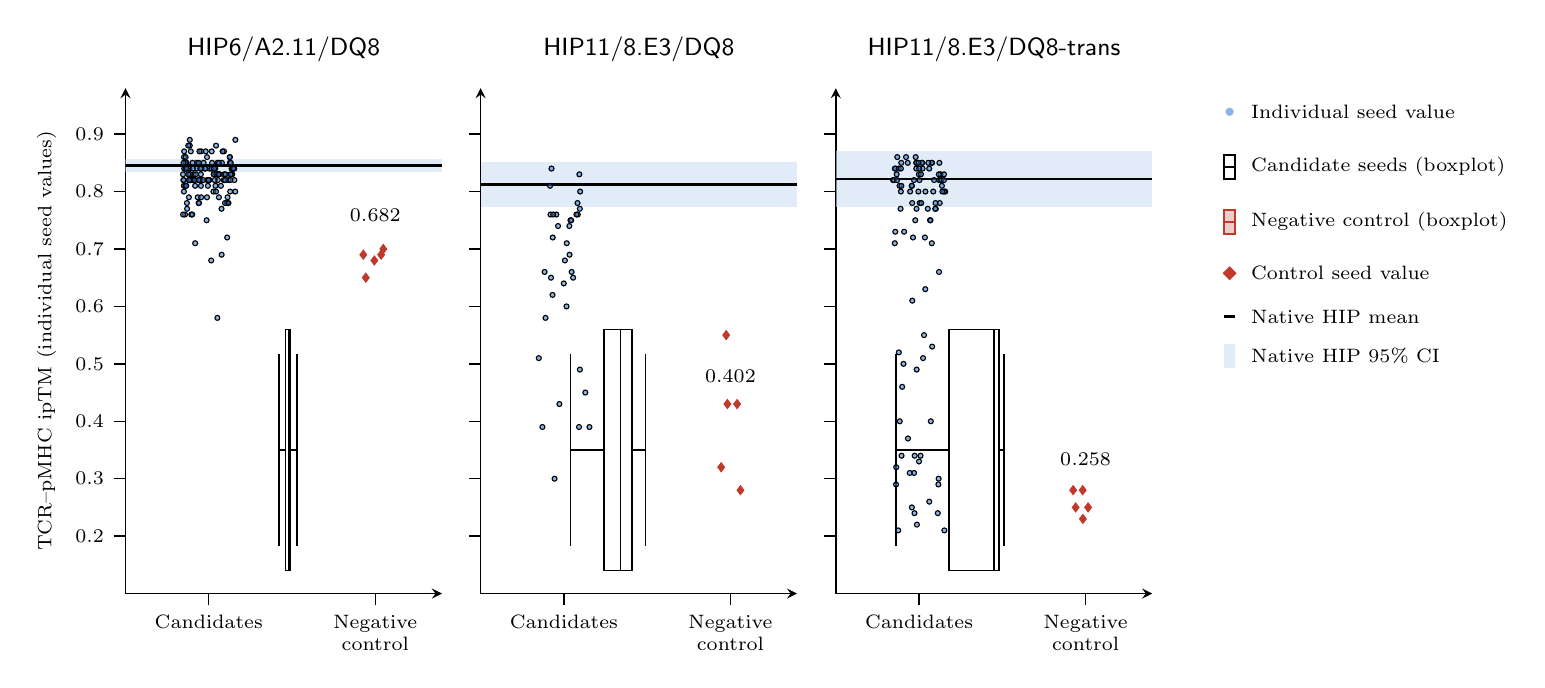
\begin{tikzpicture}[font=\sffamily]
\begin{groupplot}[
  group style={group size=3 by 1, horizontal sep=14pt, group name=distgrid},
  width=5.6cm, height=8cm,
  ymin=0.10, ymax=0.98,
  xmin=-0.15, xmax=1.75,
  axis lines=left,
  tick align=outside,
  ytick={0.2,0.3,...,0.9},
  xtick={0.35,1.35},
  xticklabels={Candidates, Negative\\control},
  x tick label style={align=center, font=\scriptsize},
  y tick label style={font=\scriptsize},
  tick style={line width=0.5pt, black},
  axis line style={line width=0.6pt},
  ytick pos=left,
]

\nextgroupplot[title={\small HIP6/A2.11/DQ8}, ylabel={TCR--pMHC ipTM (individual seed values)}, ylabel style={font=\scriptsize}]
\draw[fill=bandblue, draw=none, opacity=0.6] (axis cs:-0.15,0.8349) rectangle (axis cs:1.75,0.8571);
\draw[black, line width=1pt] (axis cs:-0.15,0.8460) -- (axis cs:1.75,0.8460);
\addplot+[boxplot prepared={lower whisker=0.77, lower quartile=0.81, median=0.83, upper quartile=0.84, upper whisker=0.88, draw position=0.35}, boxplot/box extend=0.42, fill=white, draw=black, line width=0.6pt, mark=none] coordinates {};
\addplot+[boxplot prepared={lower whisker=0.68, lower quartile=0.68, median=0.69, upper quartile=0.69, upper whisker=0.7, draw position=1.35}, boxplot/box extend=0.26, fill=seriesred, fill opacity=0.25, draw=seriesred, line width=0.6pt, mark=none] coordinates {};
\addplot[only marks, mark=*, mark size=0.9pt, draw=none, fill=seriesblue, fill opacity=0.55] coordinates {
(0.2311,0.82) (0.3498,0.82) (0.3825,0.83) (0.1992,0.82) (0.2373,0.82) (0.487,0.84) (0.2125,0.84) (0.2315,0.84) (0.4935,0.84) (0.389,0.84) (0.3081,0.84) (0.3536,0.84) (0.4021,0.85) (0.2781,0.84) (0.2341,0.84) (0.4422,0.83) (0.4045,0.82) (0.354,0.82) (0.4514,0.83) (0.3657,0.84) (0.5039,0.82) (0.2554,0.82) (0.3672,0.84) (0.3448,0.81) (0.303,0.81) (0.3793,0.83) (0.2653,0.82) (0.4467,0.82) (0.4675,0.82) (0.2312,0.82) (0.3395,0.86) (0.2787,0.85) (0.2166,0.85) (0.4767,0.85) (0.3276,0.84) (0.2373,0.83) (0.4055,0.83) (0.2547,0.84) (0.4785,0.8) (0.2595,0.82) (0.2006,0.81) (0.2542,0.82) (0.3006,0.82) (0.3401,0.82) (0.48,0.82) (0.4132,0.83) (0.2986,0.82) (0.1954,0.83) (0.2411,0.82) (0.5089,0.8) (0.3371,0.75) (0.4111,0.79) (0.2075,0.76) (0.2009,0.8) (0.4607,0.78) (0.3781,0.8) (0.2888,0.78) (0.2916,0.78) (0.2186,0.78) (0.2453,0.76) (0.1979,0.82) (0.4585,0.78) (0.3392,0.79) (0.2307,0.79) (0.4266,0.77) (0.2526,0.85) (0.2098,0.85) (0.3815,0.84) (0.4766,0.86) (0.1986,0.85) (0.4476,0.78) (0.2509,0.76) (0.2197,0.77) (0.1957,0.76) (0.2838,0.79) (0.4227,0.81) (0.3478,0.82) (0.4629,0.79) (0.2595,0.83) (0.2909,0.82) (0.2726,0.83) (0.5031,0.84) (0.4911,0.83) (0.299,0.84) (0.3295,0.84) (0.2906,0.85) (0.4289,0.85) (0.2028,0.84) (0.2116,0.84) (0.3193,0.85) (0.2684,0.71) (0.4605,0.72) (0.4274,0.69) (0.3647,0.68) (0.4017,0.58) (0.4115,0.85) (0.4399,0.82) (0.4868,0.83) (0.2379,0.83) (0.3904,0.81) (0.236,0.88) (0.3318,0.87) (0.4416,0.87) (0.4763,0.86) (0.433,0.87) (0.2013,0.86) (0.305,0.87) (0.2422,0.87) (0.5096,0.89) (0.2361,0.89) (0.2682,0.81) (0.3043,0.79) (0.2095,0.81) (0.4685,0.78) (0.3936,0.8) (0.2411,0.82) (0.3494,0.82) (0.2152,0.81) (0.3855,0.82) (0.2641,0.82) (0.2024,0.87) (0.2269,0.88) (0.3677,0.87) (0.3938,0.88) (0.2939,0.87) (0.3959,0.83) (0.3027,0.83) (0.2318,0.82) (0.2909,0.82) (0.3165,0.82) (0.482,0.85) (0.227,0.83) (0.2176,0.84) (0.3697,0.85) (0.4983,0.84) (0.4803,0.83) (0.4141,0.83) (0.2114,0.86) (0.448,0.82) (0.4087,0.83)
};
\addplot[only marks, mark=diamond*, mark size=1.6pt, draw=seriesred, line width=0.4pt, fill=seriesred] coordinates {
(1.293,0.65) (1.3444,0.68) (1.2779,0.69) (1.3983,0.7) (1.385,0.69)
};
\node[font=\scriptsize, anchor=south, fill=white, inner sep=1pt] at (axis cs:1.35,0.742) {$0.682$};

\nextgroupplot[title={\small HIP11/8.E3/DQ8}, yticklabels={}]
\draw[fill=bandblue, draw=none, opacity=0.6] (axis cs:-0.15,0.7733) rectangle (axis cs:1.75,0.8507);
\draw[black, line width=1pt] (axis cs:-0.15,0.8120) -- (axis cs:1.75,0.8120);
\addplot+[boxplot prepared={lower whisker=0.39, lower quartile=0.59, median=0.69, upper quartile=0.76, upper whisker=0.84, draw position=0.35}, boxplot/box extend=0.42, fill=white, draw=black, line width=0.6pt, mark=none] coordinates {};
\addplot+[boxplot prepared={lower whisker=0.28, lower quartile=0.32, median=0.43, upper quartile=0.43, upper whisker=0.55, draw position=1.35}, boxplot/box extend=0.26, fill=seriesred, fill opacity=0.25, draw=seriesred, line width=0.6pt, mark=none] coordinates {};
\addplot[only marks, mark=*, mark size=0.9pt, draw=none, fill=seriesblue, fill opacity=0.55] coordinates {
(0.4475,0.8) (0.4333,0.76) (0.2755,0.84) (0.4427,0.83) (0.2697,0.76) (0.2341,0.66) (0.3149,0.74) (0.3493,0.64) (0.2815,0.62) (0.3839,0.69) (0.3828,0.74) (0.2667,0.81) (0.3892,0.75) (0.3043,0.76) (0.4251,0.76) (0.2829,0.72) (0.4456,0.77) (0.3228,0.43) (0.367,0.71) (0.4055,0.65) (0.3559,0.68) (0.2724,0.65) (0.5034,0.39) (0.2207,0.39) (0.294,0.3) (0.3657,0.6) (0.1992,0.51) (0.2396,0.58) (0.4458,0.49) (0.4408,0.39) (0.3938,0.75) (0.4786,0.45) (0.4318,0.78) (0.2856,0.76) (0.3964,0.66)
};
\addplot[only marks, mark=diamond*, mark size=1.6pt, draw=seriesred, line width=0.4pt, fill=seriesred] coordinates {
(1.3244,0.55) (1.39,0.43) (1.3316,0.43) (1.2945,0.32) (1.4102,0.28)
};
\node[font=\scriptsize, anchor=south, fill=white, inner sep=1pt] at (axis cs:1.35,0.462) {$0.402$};

\nextgroupplot[title={\small HIP11/8.E3/DQ8-trans}, yticklabels={}]
\draw[fill=bandblue, draw=none, opacity=0.6] (axis cs:-0.15,0.7736) rectangle (axis cs:1.75,0.8704);
\draw[black, line width=1pt] (axis cs:-0.15,0.8220) -- (axis cs:1.75,0.8220);
\addplot+[boxplot prepared={lower whisker=0.21, lower quartile=0.528, median=0.8, upper quartile=0.83, upper whisker=0.86, draw position=0.35}, boxplot/box extend=0.42, fill=white, draw=black, line width=0.6pt, mark=none] coordinates {};
\addplot+[boxplot prepared={lower whisker=0.23, lower quartile=0.25, median=0.25, upper quartile=0.28, upper whisker=0.28, draw position=1.35}, boxplot/box extend=0.26, fill=seriesred, fill opacity=0.25, draw=seriesred, line width=0.6pt, mark=none] coordinates {};
\addplot[only marks, mark=*, mark size=0.9pt, draw=none, fill=seriesblue, fill opacity=0.55] coordinates {
(0.4109,0.84) (0.4283,0.85) (0.3691,0.85) (0.4405,0.82) (0.3333,0.85) (0.3711,0.84) (0.21,0.84) (0.3676,0.85) (0.4507,0.77) (0.4158,0.75) (0.447,0.77) (0.3488,0.83) (0.472,0.85) (0.2247,0.21) (0.4702,0.82) (0.3088,0.78) (0.2191,0.86) (0.3882,0.8) (0.3356,0.49) (0.3271,0.75) (0.4626,0.24) (0.2341,0.4) (0.3874,0.63) (0.3224,0.24) (0.359,0.34) (0.3498,0.33) (0.2329,0.81) (0.3538,0.78) (0.4659,0.29) (0.2448,0.34) (0.1937,0.82) (0.2116,0.29) (0.3371,0.22) (0.5018,0.21) (0.2042,0.71) (0.5071,0.8) (0.3615,0.83) (0.2284,0.52) (0.3239,0.34) (0.2564,0.5) (0.4185,0.75) (0.3633,0.78) (0.2821,0.85) (0.2717,0.86) (0.4674,0.3) (0.4352,0.8) (0.3296,0.86) (0.3198,0.82) (0.426,0.85) (0.5006,0.8) (0.2155,0.83) (0.2409,0.8) (0.3059,0.81) (0.3525,0.82) (0.2129,0.32) (0.2071,0.73) (0.2602,0.73) (0.3135,0.72) (0.4266,0.71) (0.3852,0.72) (0.1993,0.82) (0.2044,0.84) (0.3346,0.77) (0.47,0.66) (0.4828,0.82) (0.3068,0.25) (0.474,0.78) (0.4873,0.81) (0.3201,0.31) (0.4287,0.53) (0.3069,0.81) (0.2391,0.77) (0.3741,0.51) (0.2177,0.82) (0.4023,0.77) (0.4489,0.78) (0.4829,0.82) (0.3334,0.84) (0.2276,0.84) (0.4788,0.83) (0.4685,0.83) (0.4996,0.82) (0.3801,0.55) (0.4055,0.85) (0.3094,0.61) (0.2486,0.46) (0.2833,0.37) (0.4206,0.4) (0.294,0.31) (0.4113,0.26) (0.3507,0.84) (0.3337,0.85) (0.4996,0.83) (0.2431,0.85) (0.3459,0.8) (0.2411,0.84) (0.49,0.8) (0.3464,0.85) (0.2962,0.8) (0.2439,0.81)
};
\addplot[only marks, mark=diamond*, mark size=1.6pt, draw=seriesred, line width=0.4pt, fill=seriesred] coordinates {
(1.3651,0.25) (1.3338,0.23) (1.2903,0.25) (1.2752,0.28) (1.3326,0.28)
};
\node[font=\scriptsize, anchor=south, fill=white, inner sep=1pt] at (axis cs:1.35,0.318) {$0.258$};


\end{groupplot}

\begin{scope}[shift={(distgrid c3r1.north east)}, xshift=18pt]
\node[circle, fill=seriesblue, fill opacity=0.55, minimum size=3pt, inner sep=0, anchor=center] (l1) at (0.35cm,-0.3cm) {};
\node[font=\scriptsize, anchor=west] at (0.5cm,-0.3cm) {Individual seed value};

\draw[fill=white, draw=black, line width=0.6pt] (0.28cm,-0.85cm) rectangle (0.42cm,-1.15cm);
\draw[black, line width=0.6pt] (0.28cm,-1.0cm) -- (0.42cm,-1.0cm);
\node[font=\scriptsize, anchor=west] at (0.5cm,-1.0cm) {Candidate seeds (boxplot)};

\draw[fill=seriesred, fill opacity=0.25, draw=seriesred, line width=0.6pt] (0.28cm,-1.55cm) rectangle (0.42cm,-1.85cm);
\draw[seriesred, line width=0.6pt] (0.28cm,-1.7cm) -- (0.42cm,-1.7cm);
\node[font=\scriptsize, anchor=west] at (0.5cm,-1.7cm) {Negative control (boxplot)};

\node[rectangle, rotate=45, fill=seriesred, draw=seriesred, minimum size=3.2pt, inner sep=0, anchor=center] at (0.35cm,-2.35cm) {};
\node[font=\scriptsize, anchor=west] at (0.5cm,-2.35cm) {Control seed value};

\draw[black, line width=1pt] (0.28cm,-2.9cm) -- (0.42cm,-2.9cm);
\node[font=\scriptsize, anchor=west] at (0.5cm,-2.9cm) {Native HIP mean};

\draw[fill=bandblue, draw=none, opacity=0.6] (0.28cm,-3.25cm) rectangle (0.42cm,-3.55cm);
\node[font=\scriptsize, anchor=west, align=left] at (0.5cm,-3.4cm) {Native HIP 95\% CI};
\end{scope}

\end{tikzpicture}
\end{document}
